\subsection{مقدمه}

به دنبال پیشرفت تکنولوژی در ساخت دوربین‌های عکاسی و ورود دوربین‌های نیمه‌خودکار و خودکار به بازار، تعداد زیادی از کاربران سیستم‌های رایانه‌ای به استفاده از این تکنولوژی در ثبت تصاویر مورد علاقه خود جذب شده‌اند. دقت و کیفیت مطلوب تصویربرداری از یک سو و سهولت استفاده از دوربین‌ از سوی دیگر، باعث شده‌اند تعداد تصاویر ثبت شده توسط کاربران به طور روزافزون افزایش یابد؛ به‌طوری‌که امروزه اغلب کاربران، تعداد بی‌شماری از این تصاویر را در گوشی‌های تلفن همراه، تبلت‌ها و رایانه‌های شخصی خود نگه‌داری می‌کنند.
از جمله مشکلاتی که در اثر ایجاد این حجم وسیع از تصاویر بوجود آمده، مشکل مدیریت این تصاویر و یافتن تصاویر خاص بین مجموعه بزرگی از تصاویر موجود، است.
\\
برای دست‌یابی به سامانه‌ای که بتواند تعداد زیادی از تصاویر موجود را مدیریت نماید، ابتدا باید صحنه موجود در تصویر را به درستی درک کرد. درک صحیح از صحنه، عبارت است از بیان تصویر به نحوی که اطلاعات کلی موجود و هدف اصلی تصویر، واضح و مشخص باشد. این بیان می‌تواند شامل اجسام موجود در تصویر، رابطه مکانی بین اجسام، فعالیت به تصویر کشیده شده، شرایط محیطی موثر بر صحنه و مواردی از این دست باشد. از طرفی باید به نحوی محتوای تصاویر را بیان کرد که بتوان عملیات جستجو را بر اساس مدل بیان شده تصاویر انجام داد. در این‌صورت به‌ازای هر تصویر، یک نمونه از مدل مطابق با تصویر ایجاد و ذخیره خواهد شد. پرس‌و‌جوی\enfootnote{Query} کاربر به فضای مدل، نگاشت شده و تصویر معادل با مدلِ استخراج شده، به عنوان نتیجه جستجو نمایش داده می‌شود. علاوه بر این، مساله مدیریت تصاویر، به مساله مدیریت مدل‌های موجود کاهش داده می‌شود.
\\
تولید شرح کلی بر تصاویر\enfootnote{Holistic Image Caption}، بیان مناسبی از صحنه موجود در تصویر را ارائه می‌دهد. شرح تولید شده بر تصاویر، در قالب مجموعه‌ای از جملات زبان طبیعی\enfootnote{Natural Language Sentences} ارائه‌ می‌شود که عموما بیان‌گر اجسام موجود در صحنه‌، ارتباطات مکانی بین اجسام و اطلاعات مشخص دیگر است که در هر پژوهش می‌تواند متفاوت باشد. بنابراین، دست‌یابی به سامانه‌ای که قادر به تولید خودکار شرح کلی بر تصاویر باشد، اساسی‌ترین گام در راستای تولید نرم‌افزارهای مدیریت تصاویر است.
\\
یکی از اولین ایده‌های مطرح شده در این زمینه، با الهام از پژوهش­‌های صورت گرفته در زمینه ترجمه ماشین\enfootnote{Machine Translation}
 به‌وجود آمده‌ است که با هدف ترجمه جملات یک زبان به زبان دیگر به طور خودکار، انجام شده‌اند. در این راستا، یک جمله از زبان مبدا\enfootnote{Source Language}، با روش‌های مختلف، تبدیل به یک بردار ویژگی\enfootnote{Feature Vector} می‌شود که مشخصه‌های اصلی جمله اولیه را نمایش می‌دهد. سپس بردار ویژگی حاصل، با اعمال روش­‌های گوناگون دیگری، تبدیل به یک جمله از زبان مقصد\enfootnote{Destination Language} می­گردد که در آن تمام ویژگی‌های موجود در بردار ویژگی بیان شده‌‌اند.
با توجه به فرایند مذکور، اگر به جای جمله زبان مبدا، یک تصویر به بردار ویژگی تبدیل شده و سپس با استفاده از روش‌های موجود قبلی، بردار ویژگی حاصل به جمله زبان مقصد ترجمه شود، جمله‌ای معادل با تصویر ورودی به‌دست خواهد آمد  که بیان‌گر محتوای به تصویر کشیده شده در تصویر ورودی است\cite{xu2015show}.
\\
شرح خودکار تصاویر، توجه پژوهش‌گران بسیار زیادی را به خود جلب کرده است و فعالیت‌های متنوع و متعددی در این راستا انجام شده‌اند. علی‌رغم وجود پژوهش‌‌های فراوان و متفاوت، می‌توان یک بستر کلی برای تمام فعالیت‌های موجود در این زمینه ارائه داد. بر این مبنا، فرایند کلی که در عموم پژوهش‌های انجام‌شده، پی گرفته شده‌است، از دو بخش اساسی تشکیل می‌شود.
\begin{enumerate}
\item بازنمایی تصاویر، با استفاده از بردار ویژگی
\item تبدیل بردار ويژگی به‌دست‌آمده به جملات صحیح زبانی
\end{enumerate}


\subsection{تعریف مساله}
در این پروژه قصد داریم سامانه‌ای ارائه دهیم که قادر به تولید شرح کوتاه بر تصاویر باشد. دو دیدگاه اساسی در دست‌یابی به چنین سامانه‌ای مطرح است.
\begin{enumerate}
\item
 یافتن نقاط توجه\enfootnote{Attention Points} 
در تصاویر و تولید جملات توصیف‌کننده اجسام مستقر در این نقاط به طوری‌که توصیف جسم مستقر در نقطه توجه و اجسام مرتبط با آن در جملات تولیدی، وجود داشته باشد.
\item  تولید شرح جامع بر تصاویر به طوری‌که تمام اجسام موجود در صحنه به همراه روابط موجود بین آن‌ها توصیف شوند. 
\end{enumerate}

شرح کوتاه تولید شده در این پروژه، به معنی تولید جملاتی است که مستقیما به توصیف صحنه، اجسام موجود در صحنه و روابط بین آن­ها می­پردازند.
به طور کلی، دو چالش عمده در این پژوهش مورد توجه قرار خواهد گرفت:
\begin{enumerate}
\item  توصیف صحنه باید دقیق باشد؛ به این معنی که اجسام موجود در صحنه باید به طور دقیق از هم تفکیک شده و دسته‌بندی شوند. تصویر توصیف شده باید در قالب مناسبی بازنمایی شود که بتوان به راحتی از آن برای تولید جمله استفاده نمود.
\item  جملات تولید شده برای شرح تصویر باید به لحاظ دستور زبان، املا و معنا صحیح بوده و با تصویر مرتبط خود سازگار باشند و آن را به درستی و دقت شرح دهند.
\end{enumerate}

\subsection{درک صحنه}
مساله درک صحنه، یکی از چالش‌های بزرگ و قدیمی مطرح در زمینه بینایی ماشین است. در گذشته، هدف اغلب پژوهش‌گران از طرح این مساله، توصیف صحنه موجود در تصویر با دیدن لحظه‌ای تصویر بوده است؛ اگر‌چه امروزه، تعریف این مساله دچار تغییر شده است.
\\
به‌طور کل نمی‌توان تعریف جامع و شاملی برای درک صحنه ارائه داد. اگرچه تعاریفی عمومی ارائه شده‌اند که کلیات این مفهوم را توضیح می‌دهند. پژوهش‌‌گران در این زمینه هریک سعی در ارائه تعریفی برای این مفهوم دارند که برای کاربرد مورد نظر خود کافی و مفید باشد. به عنوان مثال، یکی از جدیدترین تعاریف برای درک صحنه در پژوهش\cite{hoiem2015guest} ارائه شده است:

\begin{enumerate}
\item [*]
«توانایی تحلیل بصری یک صحنه برای پاسخ‌دادن به سوالاتی مانند سوالات زیر:
\begin{itemize}
\item[-] چه اتفاقی در حال رخ دادن است؟
\item[-] چرا این اتفاق در حال رخ دادن است؟
\item[-] اتفاق بعدی که رخ خواهد داد، چیست؟»
\end{itemize}

\end{enumerate}

به طور کل می‌توان درک صحنه را چنین معنا کرد:
\\
\begin{enumerate}
\item [*]
درک صحنه، فرایندی است که طی آن، یک سامانه رایانه‌ای با استفاده از الگوریتم‌های موجود، اطلاعات بصری نهفته در تصاویر را استخراج کرده و در قالب مناسبی بازنمایی\enfootnote{Representation} کند به طوری‌که این اطلاعات برای توصیف صحنه کافی و مفید باشد.
\end{enumerate}

با این تعریف، اگر چه مفهوم درک صحنه کمی روشن می‌شود اما نکات مبهمی مانند این‌که چه نوع اطلاعاتی از تصویر استخراج شود، نیاز به توضیح و تفسیر بیشتری دارند. در تمام پژوهش‌های موجود در زمینه درک صحنه، که تعدادی از آن‌ها را در فصل بعدی مورد بررسی قرار خواهیم داد، تعریف اتخاذ شده برای درک صحنه، همین تعریف است با این تفاوت که اطلاعات مورد نیاز برای استخراج، در هر پژوهش، بسته به کاربرد تعریف می‌شود.
\\
موارد مختلفی که به عنوان اطلاعات لازم برای درک و توصیف صحنه، در پژوهش‌ها به چشم می‌خورد عموما شامل موارد زیر هستند:

\begin{enumerate}
\item دسته‌ صحنه\enfootnote{Scence Class} (دریا، جنگل، خیابان، کلاس درس و مواردی از این دست)
\item دسته‌ اجسام\enfootnote{Object Class} موجود در صحنه (صندلی، مرد، گربه و مواردی از این دست)
\item ارتباط مکانی بین اجسام موجود (بالا، کنار، پشت و مواردی از این دست)
\item رخدادی\enfootnote{Event} که در صحنه در حال اتفاق است (مانند نشستن، دویدن، کارکردن و مواردی از این دست)
\end{enumerate}

\subsubsection{پژوهش‌های انجام‌شده در زمینه درک صحنه توسط مغز انسان}
مساله درک صحنه، مانند بیشتر مسائل موجود در زمینه بینایی ماشین، الهام گرفته از نحوه رفتار انسان‌ها است. اغلب انسان‌ها با دیدن یک تصویر قادرند توصیف کامل و دقیقی از آن تصویر ارائه دهند که شامل تمام نکات لازم و ضروری نهفته در تصویر باشد. در بیشتر موارد، زمان مورد نیاز برای مغز انسان به منظور پردازش یک تصویر و توصیف آن، زمان بسیار کم و ناچیزی است. این مطلب، این ایده را در ذهن تداعی می‌کند که بخش قابل توجهی از اطلاعات مورد نیاز از هر تصویر، در اولین لحظاتی که تصویر به مغز می‌رسد (در نگاه اول) قابل استخراج است. بنابراین سامانه‌های رایانه‌ای باید قادر باشند با الگو گرفتن از مغز انسان، در کوتاه‌ترین زمان ممکن، اطلاعات کافی و مفید نهفته در تصویر را استخراج کرده و صحنه به نمایش کشیده شده در تصویر را توصیف کنند.
\\
این فرض که مغز انسان می‌تواند در کوتاه‌ترین زمان ممکن، بیشترین حجم اطلاعات تصویر را به درستی استخراج نماید، توسط پژوهش‌گران متعددی مورد ارزیابی قرار گرفته است. از جمله اولین پژوهش‌هایی که به بررسی این فرض پرداخته‌اند می‌توان به 
\cite{potter1976short}
و
\cite{potter2002recognition}
اشاره کرد. در این‌ پژوهش‌ها، با نشان دادن تصاویر به صورت دنباله‌ای\enfootnote{Image Series} به مجموعه‌ای از افراد، از آن‌ها خواسته شده تا بهترین و دقیق‌ترین توصیفی را که می‌توانند، برای تصاویری که دیده‌اند، بازگو کنند. در این دو پژوهش نتیجه گرفته شده است که انسان می‌تواند یک تصویر معمولی را در بازه زمانی کمتر از ۲۰۰ میلی‌ثانیه، تشخیص داده و آن را توصیف کند. اگرچه این زمان برای تشخیص و توصیف یک تصویر کافیست، زمان مورد نیاز برای به‌خاطرسپاری تصویر بسیار بیشتر از این مقدار است.
\\
در پژوهش\cite{fei2007we}
آزمایش دیگری انجام شده که از اهمیت بسیاری برخوردار است. در پژوهش‌های قبلی، افرادی که تصاویر را توصیف می‌کردند، درباره موضوع کلی تصاویر اطلاعاتی داشتند. اما در این آزمایش، تصاویر مختلفی از دنیای واقعی که محدود به شرایط خاصی نبوده‌اند، بدون ارائه پیش‌فرض درباره موضوع، به افراد نمایش داده شده و از آن‌ها خواسته شده که تصویر را به بهترین شکل توصیف کنند. آزمایشات در این پژوهش، در دو مرحله انجام شده‌اند.
\begin{enumerate}
\item توسط یک رایانه، تصاویر متعددی در بازه‌های زمانی متفاوت به افراد نمایش داده می‌شوند و پس از اتمام زمان نمایش هر تصویر، یک ماسک بصری، تصویر را می‌پوشاند. در این حالت از افراد خواسته‌شده  است که بهترین توصیف ممکن از تصویر را تایپ کنند. شرایط محیطی آزمایشات مطابق با استانداردها رعایت شده است. هر تصویر به طور تصادفی بین 27 الی 500 میلی ثانیه روی نمایش‌گر نمایش‌داده شده و سپس یک ماسک روی تصویرقرار گرفته و افراد فرصت دارند تا توصیف خود را از تصویر، بنویسند.


\begin{figure}[H]
\center
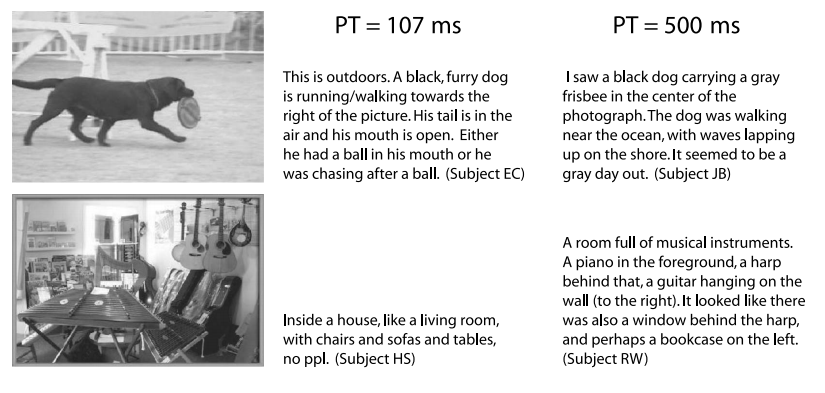
\includegraphics[scale=0.5]{./Imgs/fei2007we_res2.png}
\caption[نمونه توصیف‌های افراد برای تصاویر]{نمونه‌ توصیف‌های افراد برای تصاویر\cite{fei2007we}}
\label{fig:f2007we1}
\end{figure}



\item در این مرحله، آزمایش روی افراد متفاوتی انجام شده‌است. این گروه افراد موظفند پس از دیدن تصاویر، به بهترین شکل ممکن آن‌ها را دسته‌بندی کنند. برخلاف افراد شرکت‌کننده در آزمایش قبلی  که می‌توانستند به هر شکلی اطلاعات استخراج شده را بنویسند، به افراد حاضر در این گروه یک فرم مشخص از دسته‌اطلاعات مطلوب داده شده است که افراد موظفند آن را براساس محتوای تصویری که دیده‌اند، پر کنند. شکل\ref{fig:f2007we2}
ساختار مطلوب پاسخ افراد را در این آزمایش نمایش می‌دهد.

\begin{figure}[H]
\center
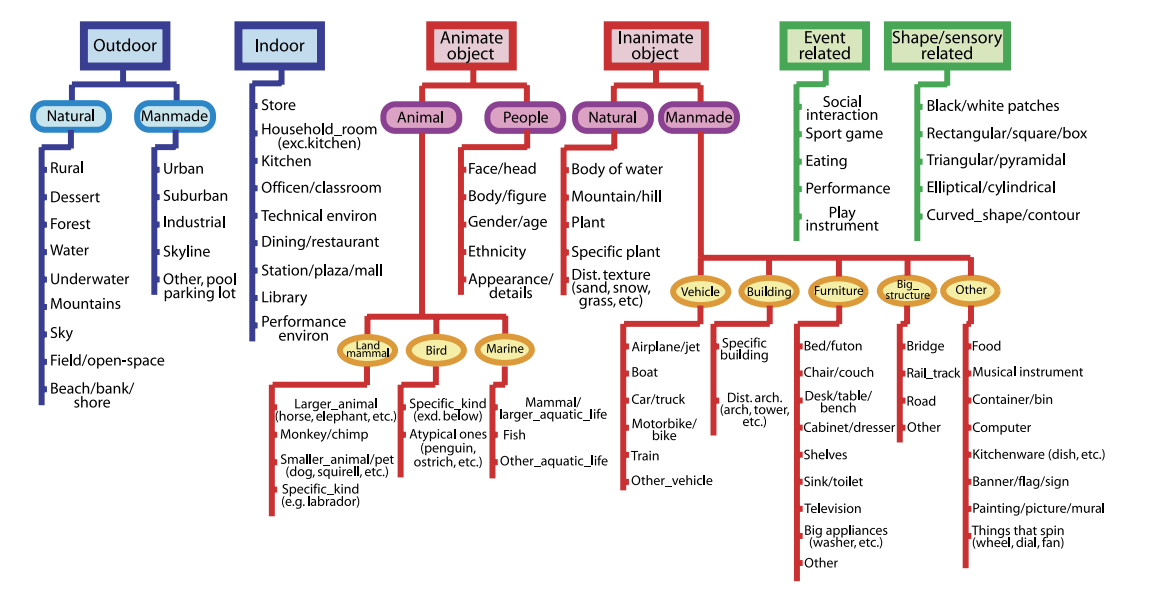
\includegraphics[scale=0.4]{./Imgs/fei2007we_exp1.png}
\caption{ساختار مطلوب اطلاعات استخراج‌شده از تصاویر\cite{fei2007we}}
\label{fig:f2007we2}
\end{figure}

این ساختار با تحلیل پاسخ‌های جمع‌آوری شده از آزمایش اول استخراج شده است و شامل انواع مختلفی از اطلاعات است که افراد در آزمایش اول به آن اشاره‌کرده‌اند.





\end{enumerate}


شکل\ref{fig:f2007wd}
چند نمونه از تصاویر مورد استفاده در آزمایشات این پژوهش را نمایش می‌دهد. این تصاویر از اینترنت استخراج شده‌اند. برای استخراج این تصاویر از فضای اینترنت، از یک گروه افراد شامل ۱۰ نفر که با موضوع پژوهش آشنا نبوده‌اند خواسته‌شده تا هر یک، نام ۵ دسته صحنه مختلف را به طور تصادفی بنویسند. پس از حذف نام‌های تکراری، ۲۵ الی ۳۰ نام منحصربه‌فرد باقی مانده‌است. سپس تصاویر مربوط به هریک از این نام‌ها توسط موتور جستجوی گوگل استخراج شده و ۳ الی ۶ تصویر از صفحات اولیه نتایج به عنوان تصاویر نمونه انتخاب شده‌اند.

\begin{figure}[H]
\centering
	\subfigure[چند نمونه از تصاویر در محیط باز]{
		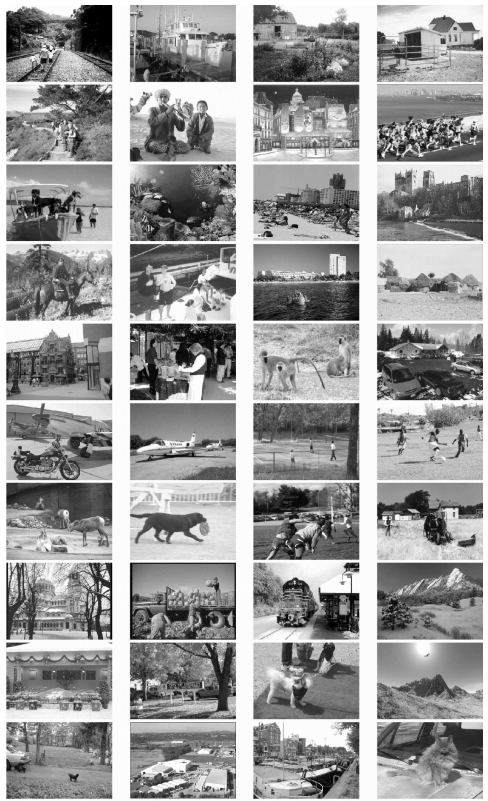
\includegraphics[scale=0.4]{./Imgs/fei2007we_data1.png}
	}	
	\hspace*{1mm}
	\subfigure[چند نمونه از تصاویر در محیط بسته]{
		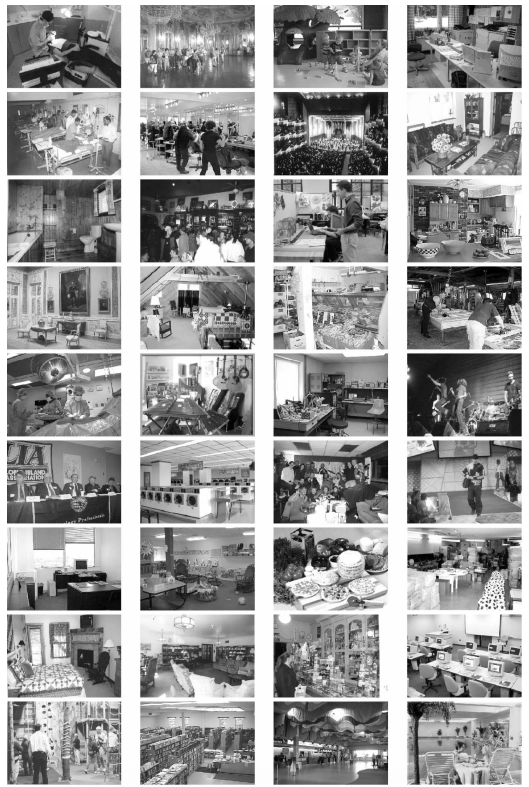
\includegraphics[scale=0.4]{./Imgs/fei2007we_data2.png}
	}
\caption{تصاویر دنیای واقعی مورد استفاده در آزمایشات\cite{fei2007we}}
\label{fig:f2007wd}
\end{figure}


ارزشمندترین نکته درباره پژوهش انجام‌شده، یافته‌های آن است. این پژوهش نکاتی را در مورد توانایی مغز انسان در توصیف صحنه روشن می‌کند که حائز اهمیت هستند. در ادامه این نتایج را بررسی خواهیم کرد.
\subsubsection{نتایج به‌دست‌ آمده از آزمایشات}
\begin{enumerate}
\item
حداکثر زمان لازم برای مغز انسان به منظور درک صحنه، برابر با 500 میلی‌ثانیه است.
\item
این مدت زمان، برای صحنه‌های ساده‌ و بدون پیچیدگی، به حدود ۱۰۰ میلی‌ثانیه می‌رسد. به عنوان نمونه در شکل\ref{fig:f2007we1} تصویر اول که دارای پیچیدگی‌های کمتری نسبت به تصویر دوم است در مدت زمان ۱۰۷ میلی‌ثانیه، به‌طور کامل توصیف شده‌است در صورتی‌که تصویر دوم که به نسبت، پیچیده‌تر است، مدت‌زمان بیشتری برای توصیف نیاز داشته‌است.
\item
با استفاده از ساختارمندسازی پاسخ‌های افراد در آزمایش دوم و اطلاعات جمع‌آوری شده در درخت پاسخ‌ها (که در شکل\ref{fig:f2007we2} نمایش‌ داده شده است) و میانگین‌گیری روی تمام تصاویر، نمودارهای مقایسه‌ای برای مدت زمان 107 میلی‌ثانیه و 500 میلی‌ثانیه ایجاد شده‌ است. شکل\ref{fig:f2007res3}
نمودارهای مقایسه‌ای را نمایش‌ می‌دهد. در این نمودارها، میله‌های قرمز نشان‌دهنده نتایج برای زمان ۵۰۰ میلی‌ثانیه و میله‌های آبی نمایش‌دهنده نتایج برای حالت ۱۰۷ میلی‌ثانیه هستند.
در دو نمودار اول (نمودارهای بالا سمت راست و بالا سمت چپ) تشخیص و استخراج اطلاعات مربوط به اجسام مختلف بسته به متحرک بودن\enfootnote{Animated} یا متحرک نبودن\enfootnote{Inanimated} آن‌ها، در نمودار سوم (نمودار پایین سمت چپ) تشخیص و استخراج اطلاعات مربوط به صحنه موجود در تصویر و در نمودار چهارم‌ (نمودار پایین سمت راست) تشخیص و استخراج اطلاعات مربوط به رخداد موجود در تصویر، مورد بررسی قرار گرفته‌اند.


\begin{figure}[H]
\center
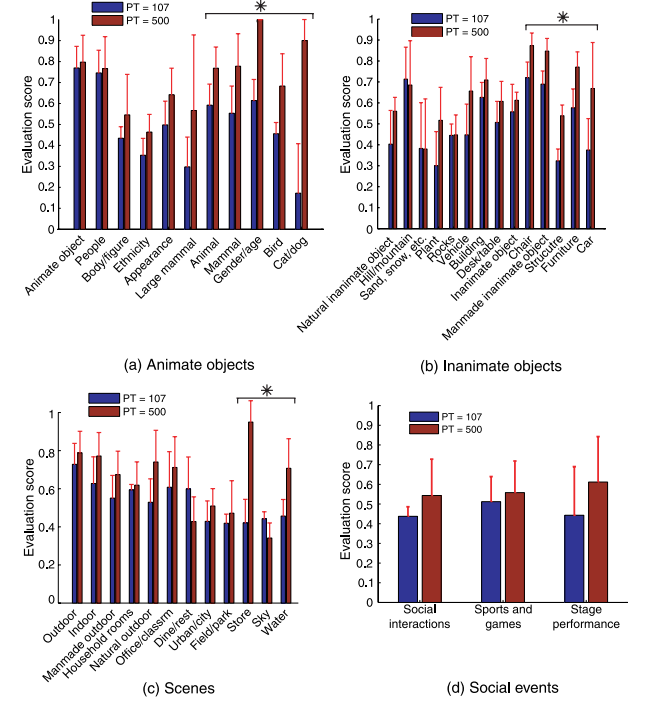
\includegraphics[scale=0.6]{./Imgs/fei2007we_res3.png}
\caption[نمودار مقایسه‌ای عملکرد مغز در درک صحنه]{نمودارهای مقایسه‌ای عملکرد مغز انسان در درک صحنه در بازه‌های زمانی ۱۰۷ و ۵۰۰ میلی‌ثانیه\cite{fei2007we}}
\label{fig:f2007res3}
\end{figure}

همان‌طور که مشخص است، مدت زمان ۱۰۷ میلی‌ثانیه برای مغز انسان، زمان بهینه برای توصیف صحنه است. تفاوت‌های بین نتایج در اکثر موارد، جزئی و در مقابل تفاوت زمانی موجود، بسیار کوچک هستند.
به علاوه، در تمام مواردی که نیاز به اطلاعات کلی از تصویر وجود دارد، تفاوت بین دو بازه زمانی چندان چشم‌گیر نیست، اما در مواردی که برای تشخیص نیاز به دانستن جزئیات بیشتر از تصویر وجود دارد (مانند سن، جنسیت و نوع حیوان) تفاوت بین دو زمان، قابل ملاحظه است.
\\
همین‌طور با مقایسه تفاوت عملکرد بین حالات متحرک بودن و متحرک نبودن اجسام، فواصل موجود در نمودارها قابل ملاحظه می‌شود. در حالت کلی، تفاوت بین عملکرد مغز در دو بازه، در حالتی‌که اجسام ساکن در تصویر وجود دارند به مراتب کمتر از حالتی است که اجسام موجود در تصویر، متحرک باشند.
\end{enumerate}

شکل\ref{fig:f2007res4} نمونه دیگری از نتایج به‌دست‌آمده از آزمایشات را در مدت‌زمان‌های مختلف نمایش ‌می‌دهد.



\begin{figure}[H]
\center
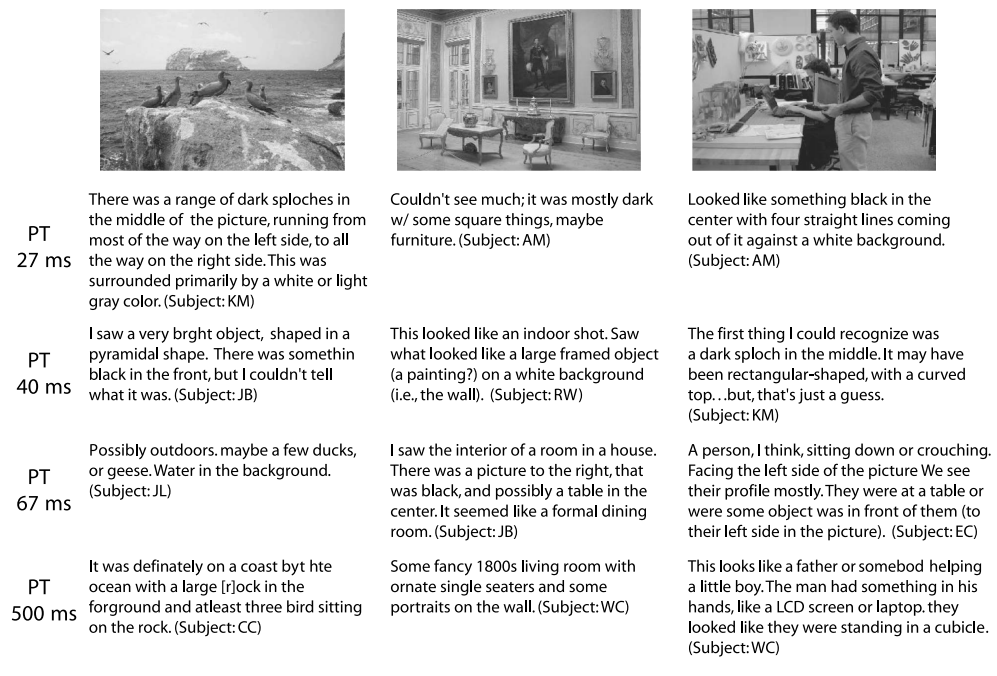
\includegraphics[scale=0.4]{./Imgs/fei2007we_res4.png}
\caption{نمونه‌ای از نتایج به‌دست‌آمده از آزمایشات\cite{fei2007we}}
\label{fig:f2007res4}
\end{figure}
%%%%%%%%%%%%%%%%%%%%%%%%%%%%%%%%%5

\subsection{جمع‌بندی}
‫با توجه به افزایش چشم‌گیر تعداد تصاویر مورد استفاده کاربران در فضاهای مجازی و همین‌طور با در نظر گرفتن گرایش روزافزون کاربران به ذخیره‌سازی تصاویر در رایانه‌های شخصی، مساله مدیریت این تصاویر و یافتن تصاویر خاص بین مجموعه تصاویر موجود، به یکی از مسائل مهم و پرکاربرد در زمینه بینایی ماشین تبدیل شده‌ است. گام اساسی در این راستا، دست‌یابی به سامانه‌ای است که قادر به تولید خودکار شرح برای تصاویر باشد. شرح این تصاویر که در قالب جملات زبان طبیعی ارائه می­شود باید علاوه بر سازگاری با موضوع تصویر و توصیف صحیح صحنه، به لحاظ دستور زبان و معنا صحیح و کامل باشد. 
\\
فرایند تولید خودکار شرح برای تصاویر، از دو مرحله اصلی تشکیل می‌شود:
\begin{enumerate}
\item نگاشت تصویر ورودی به فضای بردار ویژگی‌ها (درک صحنه)
\item تولید جملات زبان طبیعی مبتنی بر محتوای بردار ویژگی‌ها 
\end{enumerate}

مساله درک صحنه، یکی از چالش‌ بر‌انگیزتزین مسائل در زمینه بینایی ماشین است. با این وجود، تا کنون تعریف دقیق و کاملی از این مفهوم ارائه نشده است. به طور کلی می‌توان درک صحنه را فرایندی دانست که طی آن اطلاعات بصری موجود در تصویر استخراج شده و در قالب خاصی بازنمایی می‌شوند. میزان و نوع این اطلاعات را نمی‌توان به طور کلی تعریف کرد. حوزه تعریف اطلاعات و کیفیت مطلوب آن‌ها بسته به کاربرد در هر حوزه تعریف می‌شود.
\\
در بین پژوهش‌های مربوط به تولید خودکار شرح برای تصاویر، انواع اطلاعات مطلوب، عموما شامل موارد زیر می‌شود:


\begin{enumerate}
\item دسته‌ صحنه
\item دسته‌ اجسام
\item ارتباط مکانی بین اجسام موجود
\item رخدادی که در صحنه در حال اتفاق است
\end{enumerate}

پژوهش‌گران از گذشته بر این عقیده بوده‌اند که مغز انسان در اولین لحظات مشاهده یک تصویر، قادر است اطلاعات کافی و مفید برای درک صحنه را استخراج کند. پژوهش‌های متعددی در این زمینه انجام شده‌اند که هریک به بررسی جوانب خاصی از این فرضیه پرداخته‌اند. به عنوان نمونه، پژوهش\cite{potter1976short}
و 
\cite{potter2002recognition} 
با استفاده از دنباله‌های تصاویر، مدت زمان مورد نیاز برای مغز انسان به جهت درک صحنه را کمتر از 200 میلی‌ثانیه تخمین زده‌اند.
\\
در پژوهش\cite{fei2007we}، یک آزمایش دو مرحله‌ای برای بررسی تاثیر مدت زمان مشاهده تصاویر بر عملکرد مغز در توصیف صحنه، انجام شده است. در این آزمایش که در دو مرحله انجام شده، ابتدا گروهی از افراد با دیدن تصاویر در مدت‌زمان بین 27 تا 500 میلی‌ثانیه، موظف به توصیف تصویر بوده‌اند. سپس گروه دیگری از افراد با دیدن تصاویر در مدت‌زمان‌های مختلف، ملزم به پر کردن فرم از پیش تعیین‌شده‌ای بودند که با توجه به پاسخ‌های به‌دست‌آمده از آزمایش اول، تدوین شده است.
\\
نتایج این آزمایشات نشان می‌دهد، مدت زمان ۱۰۷ میلی‌ثانیه برای تشخیص و بخش قابل توجهی از اطلاعات موجود در تصویر کافیست؛ اگرچه، در مواردی که دق به جزئیات ضروری است‌ (مانند تشخیص سن، جنسیت، نوع حیوان) و برای تشخیص و استخراج اطلاعات اجسام متحرک، مدت‌زمان 500 میلی‌ثانیه، بهبود قابل توجهی در عملکرد مغز ایجاد می‌کند.